\section{Batch and scheduling}

\subsection{Objectives}

	\begin{frame}
		\frametitle{Objectives}
		
		Our worker is fine, but induces too much stress on the system.We now want to deploy it as a batch.
		
		\bigskip
		As such, we want to be able to schedule it.
		
		\bigskip
		We are now going to create a batch performing the same task as our worker.
	\end{frame}

	\begin{frame}
		\frametitle{What kind to use to deploy our application}
		
		\begin{center}
		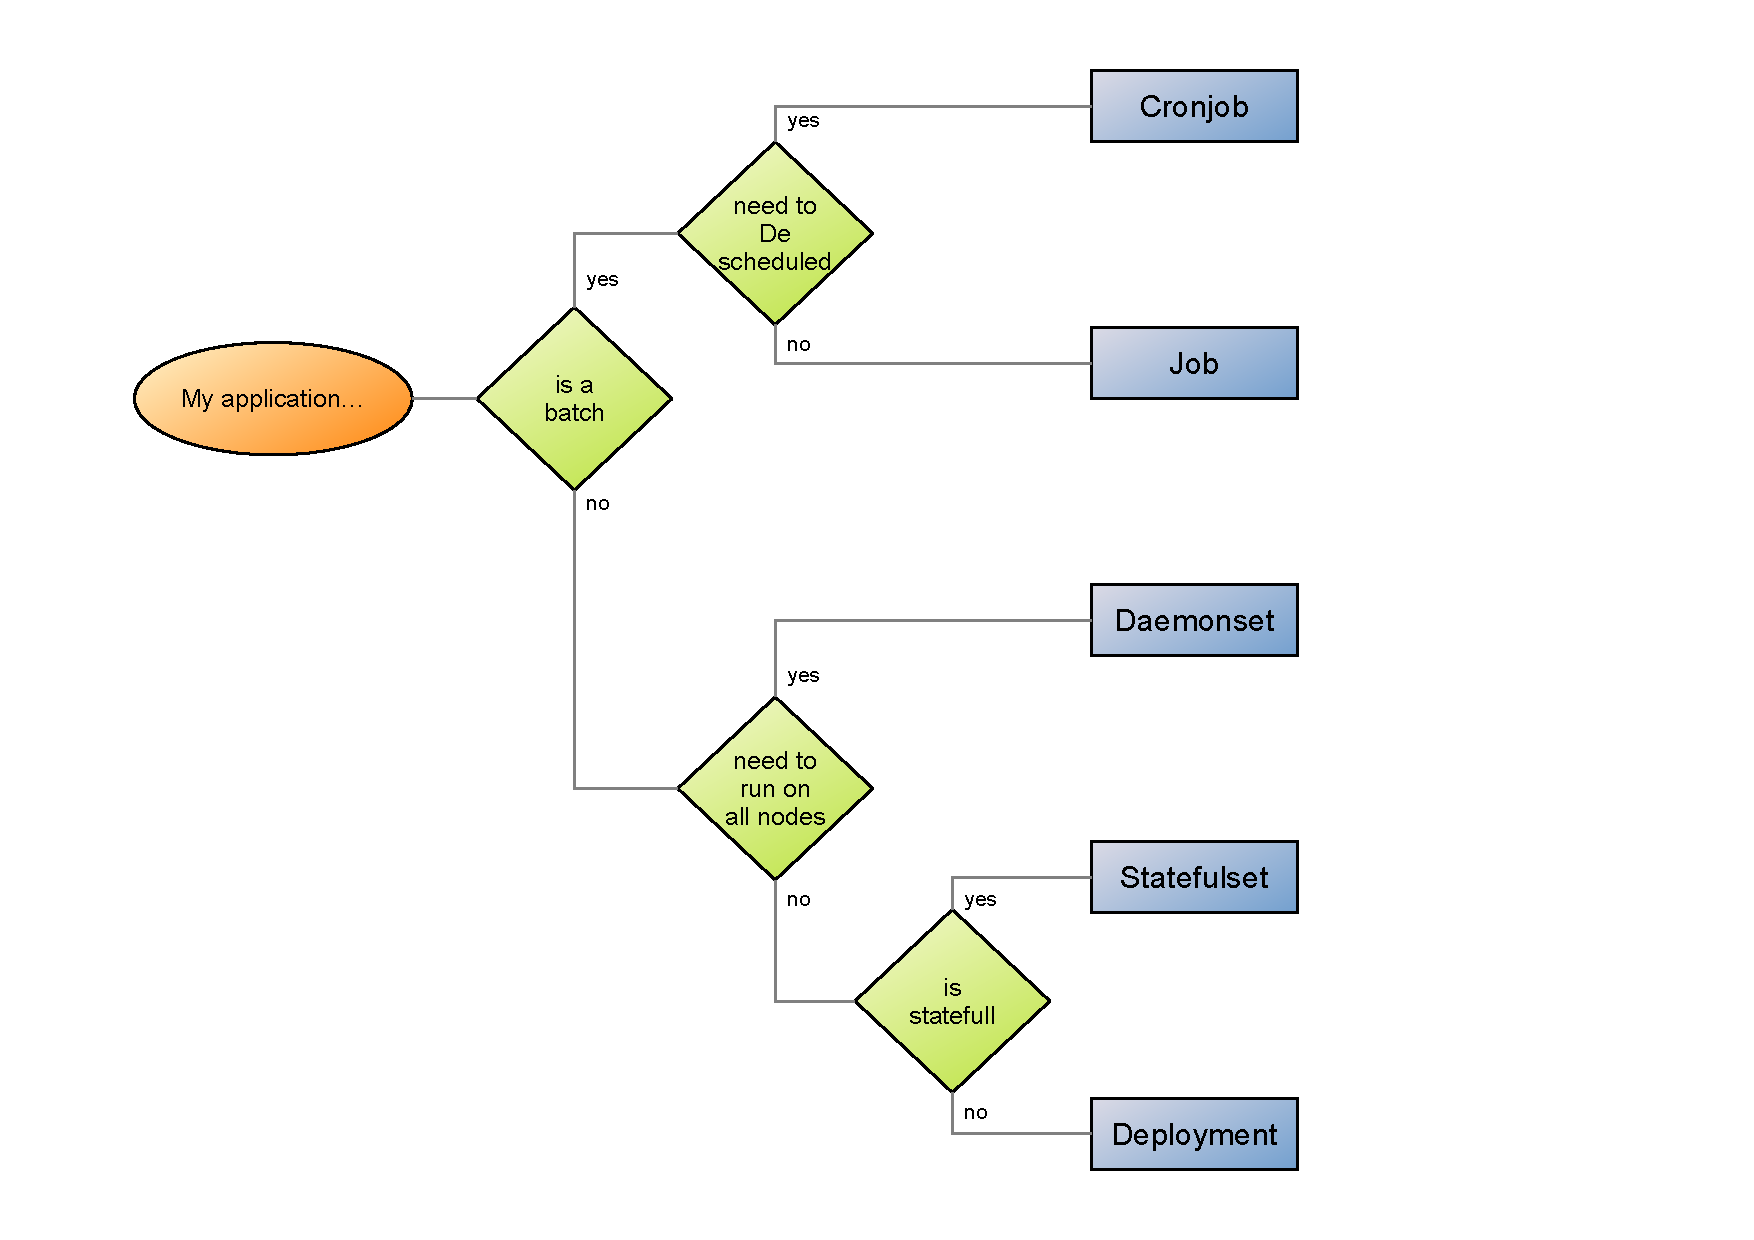
\includegraphics[height=6.8cm]{../../../resources/color/choiceDeploymentType.pdf}
		\end{center}
	\end{frame}
		
\subsection{Creating a batch in kubernetes}		
		
	\begin{frame}[fragile]
		\frametitle{Creating the batch}
		
		Beside the folder \verb!worker!, create a folder \verb!batch!.
		
		\bigskip
		Create the batch itself:
		\begin{block}{batch/batch.sh}
			\begin{verbatim}
				echo "I'm Humphrey and it is $(date)"
			\end{verbatim}
		\end{block}
		Now, each execution is unitary.
	\end{frame}
	
	\begin{frame}[fragile]
		\frametitle{Exercise}
		
		Build and run in docker an image \verb|tinkou/batch:v1| containing this batch.
	\end{frame}

	\begin{frame}[fragile]
		\frametitle{A solution}
		
		\begin{block}{batch/Dockerfile}
			\begin{verbatim}
				FROM alpine
				
				COPY batch.sh .
				RUN chmod u+x batch.sh
				
				CMD /batch.sh
			\end{verbatim}
		\end{block}
		
		\begin{block}{Command terminal in folder batch}
			\begin{verbatim}
				docker build -t tinkou/batch:v1 .
				docker run tinkou/batch:v1
			\end{verbatim}
		\end{block}
	\end{frame}
				
	\begin{frame}[fragile]
		\frametitle{Creating our first CronJob}
		
		\begin{block}{batch/cronjob.yaml}
			\begin{tiny}
				\begin{verbatim}
					apiVersion: batch/v1beta1
					kind: CronJob
					metadata:
					  name: my-batch
					spec:
					  schedule: "* * * * *"
					  jobTemplate:
					    spec:
					      template:
					        metadata:
					          labels:
					            tinkou: batch
					        spec:
					          containers:
					          - name: runner
					            image: tinkou/batch:v1
					            env:
					            - name: NAME
					              value: Chem
					          restartPolicy: Never
				\end{verbatim}
			\end{tiny}
		\end{block}
	\end{frame}
	
	\begin{frame}[fragile]
		\frametitle{Creating our first CronJob}
		
		\begin{block}{Logs terminal}
			\begin{verbatim}
				stern -l tinkou=batch
			\end{verbatim}
		\end{block}
		
		\begin{block}{Monitor terminal}
			\begin{verbatim}
				watch kubectl get all
			\end{verbatim}
		\end{block}
		
		\begin{block}{Command terminal}
			\begin{verbatim}
				kubectl apply -f cronjob.yaml
			\end{verbatim}
			Wait for a few batches to run…
			\begin{verbatim}
				kubectl logs -l tinkou=batch
			\end{verbatim}
		\end{block}
	\end{frame}

	\begin{frame}
		\frametitle{Conclusions}
		
		\begin{block}{Conclusions}
			\begin{itemize}
				\item[$\bullet$] CronJob are easy to defined
				\item[$\bullet$] stern is less adapted than a standard kubectl logs for jobs
			\end{itemize}
		\end{block}
		
		\begin{block}{CronJobs useful options}
			\begin{itemize}
				\item[$\bullet$] A field .spec.suspend suspend the scheduling of a CronJob
				\item[$\bullet$] Jobs in error aren't removed
				\item[$\bullet$] The history limit of successful jobs can be set
			\end{itemize}
		
		\end{block}
	\end{frame}
	
\subsection{Using a layer based configuration}	
	
	\begin{frame}
		\frametitle{Exercise}
		
		Modify the configuration to use kustomize and skaffold with:
		\begin{itemize}
			\item[$\bullet$] a base configuration similar as the current one
			\item[$\bullet$] a local configuration for minikube with NAME=Dolph
		\end{itemize}
	\end{frame}
	
	\begin{frame}[fragile]
		\frametitle{A solution}
		
		\begin{block}{Folder tree in batch folder}
			\begin{small}
				\begin{verbatim}
					batch
					|- batch.sh
					|- Dockerfile
					|- kube
					   |- base
					   |  |- conf.env
					   |  |- cronjob.yaml
					   |  |- kustomization.yaml
					   |- local
					      |- conf.yaml
					      |- kustomization.yaml
				\end{verbatim}
			\end{small}
		\end{block}

		\begin{block}{batch/kube/base/conf.env}
			\begin{small}
				\begin{verbatim}
					NAME=Humphrey
				\end{verbatim}
			\end{small}
		\end{block}

	\end{frame}
	
	\begin{frame}[fragile]
		\frametitle{A solution}
				
		\begin{block}{batch/kube/base/cronjob.yaml}
			\begin{tiny}
				\begin{verbatim}
					apiVersion: batch/v1beta1
					kind: CronJob
					metadata:
					  name: my-batch
					spec:
					  schedule: "* * * * *"
					  jobTemplate:
					    spec:
					      template:
					        metadata:
					          labels:
					            tinkou: batch
					        spec:
					          containers:
					          - name: runner
					            image: tinkou/batch:v1
					            envFrom:
					            - configMapRef:
					                name: batch
					          restartPolicy: Never
				\end{verbatim}
			\end{tiny}
		\end{block}
	\end{frame}
	
	\begin{frame}[fragile]
		\frametitle{A solution}

		\begin{block}{Command terminal in folder batch/kube/base}
			\begin{verbatim}
				kustomize create --resources cronjob.yaml
				kustomize edit add configmap batch \
				                             --from-env-file conf.env
			\end{verbatim}
		\end{block}
	\end{frame}
	
	\begin{frame}[fragile]
		\frametitle{A solution}
		
		\begin{block}{batch/kube/local/conf.yaml}
			\begin{verbatim}
				apiVersion: v1
				kind: ConfigMap
				metadata:
				  name: batch
				data:
				  NAME: Dolph
			\end{verbatim}
		\end{block}
	\end{frame}
	
	\begin{frame}[fragile]
		\frametitle{A solution}
		
		\begin{block}{Command terminal in folder batch/kube/local}
			\begin{verbatim}
				kustomize create --resources ../base
				kustomize edit add patch conf.yaml
			\end{verbatim}
		\end{block}
	\end{frame}
	
	\begin{frame}[fragile]
		\frametitle{A solution}
		
		\begin{block}{batch/skaffold.yaml}
			\begin{footnotesize}
				\begin{verbatim}
					apiVersion: skaffold/v1beta12
					kind: Config
					build:
					  artifacts:
					  - image: tinkou/batch
					deploy:
					  kustomize:
					    path: kube/base
					profiles:
					- name: local
					  activation:
					  - kubeContext: minikube
					  deploy:
					    kustomize:
					      path: kube/local
				\end{verbatim}
			\end{footnotesize}
		\end{block}
	\end{frame}
	
	\begin{frame}[fragile]
		\frametitle{A solution}
		
		\begin{block}{Command terminal in folder batch}
			\begin{verbatim}
				skaffold run
			\end{verbatim}
		\end{block}
		
		\bigskip
		
		Take a quick look at the scheduling options and logs:
		\begin{block}{Command terminal}
			\begin{verbatim}
				kubectl describe cronjob my-batch
			\end{verbatim}
		\end{block}
		
		\bigskip
		
		Clean after working:
		\begin{block}{Command terminal in folder batch}
			\begin{verbatim}
				skaffold delete
			\end{verbatim}
		\end{block}
	\end{frame}
	
	\begin{frame}
		\begin{center}
			Questions?
		\end{center}
	\end{frame}